\documentclass[a4paper,10pt]{scrartcl}
\usepackage[utf8]{inputenc}
\usepackage[T1]{fontenc}
\usepackage[naustrian]{babel}
\usepackage{lmodern}
\usepackage{graphicx}
\usepackage{hyperref}
%\usepackage{tabularx}
%\usepackage{amsmath}

%opening
\title{HCI Meilenstein 3}
\subtitle{Elektronisches Curriculum}
\author{Team 1 \\Pascal Attwenger, Philipp Hiermann, Sandra Markhart}

\begin{document}

\maketitle

\section{Usability Test Aufgaben}

\subsection{Aufgabe 1}

\subsubsection*{Ziel:}
 
Der User soll herausfinden welche Fächer er im 1. Semester absolvieren muss und kann.
 
\subsubsection*{Beschreibung:}

Du fängst nächstes Semester an Medieninformatik zu studieren. Für welche Fächer sollst du dich anmelden?
 
\subsection{Aufgabe 2}

\subsubsection*{Ziel:}

Der User soll seine Note abfragen.

\subsubsection*{Beschreibung:}

Du hast vor 2 Wochen die Vorlesungsprüfung zu VO Netzwerktechnologien abgelegt. Hast du bereits eine Note erhalten? Wenn ja welche?

\subsection{Aufgabe 3}

\subsubsection*{Ziel:}

Der User soll seinen Notendurchschnitt herausfinden.

\subsubsection*{Beschreibung:}

Du studierst an der Universität Wien und willst wissen ob du dich für ein Leistungsstipendium eignest. Das Stipendium verlangt einen Notendurchschnitt von
1,8. Kannst du ein Leistungsstipendium erhalten?


\section{Interviewleitfaden}

\subsection{Vorinterview}

\begin{itemize}
 \item Was sind deine Erfahrungen mit den aktuellen IT-Systemen im Studium? (univis, TISS, etc.)
 \item Was sind deiner Meinung nach die größten Schwächen dieser Systeme?
 \item Was würdest du dir von einem neuen System erwarten?
\end{itemize}

\subsection{Ad Aufgabe 1}

\begin{itemize}
 \item Ist dir klar, was die StEOP generell ist?
 \item Angenommen, du würdest nur die unbedingt vorausgesetzten StEOP-Fächer belegen wollen -- welche wären das?
 \item Angenommen, du würdest alles belegen wollen, was im ersten Semester überhaupt möglich ist -- welche Fächer wären jetzt zusätzlich dabei?
 \item Was hältst du von der Darstellungsart, bei der immer nur genau ein Modul angezeigt wird?
 \item Vergleiche die Sortierung nach Modulgruppen mit der nach Semestereinteilung -- welche erscheint dir vernünftiger, und wieso?
 \item Wirf noch einen Blick auf die anderen Rubriken des eCurriculums (Allgemeines, Ausland, etc.) -- macht diese Aufteilung so für dich Sinn? Was würdest du evtl. anders gruppieren?
 \item Hast du noch andere Anmerkungen zu dieser Oberfläche?
\end{itemize}

\subsection{Ad Aufgabe 2}

\begin{itemize}
 \item Ist dir klar, was es mit dem ``Persönlichen Plan'' auf sich hat?
 \item Ist dir der Unterschied zwischen Modulnote und LV-Note bewusst?
 \item Was bedeuten die kleinen Symbole (``Hakerl'') in der Tabellen-Übersicht?
 \item Kann diese Art der Darstellung die Listen-Ansicht der Prüfungsleistungen ersetzen oder nur ergänzen?
 \item Kannst du dir vorstellen, dass diese Art des Semesterplans auch für dein Studium möglich wäre? Wo wären eventuelle Probleme?
 \item Hast du noch andere Anmerkungen zu dieser Oberfläche?
\end{itemize}

\subsection{Ad Aufgabe 3}

\begin{itemize}
 \item Findest du die automatische Berechnung des Notenschnitts sinnvoll? Wozu braucht man diese Information?
 \item Welche anderen Statistiken fändest du praktisch?
 \item Was hältst du von der Studienfortschrittsanzeige?
 \item Hast du noch andere Anmerkungen zu dieser Oberfläche?
\end{itemize}

\subsection{Abschlussfragen}

\begin{itemize}
 \item Was sind deine allgemeinen Eindrücke vom System?
 \item Wie gut konntest du dich orientieren?
 \item Was hat dir besonders gut/schlecht gefallen?
 \item Wurden deine Erwartungen an das System erfüllt?
 \item Hast du Verbesserungsvorschläge?
\end{itemize}

\section{Abschlussinterview}



\section{Bericht}

\subsection{Aufgabe 1}

\subsection{Aufgabe 2}

\subsection{Aufgabe 3}

\subsection{Gesamteinschätzung}

\subsection{Verbesserungsvorschläge}

\section{Weiterentwickelter Prototyp}

\begin{description}
 \item[Url:] \url{http://wwwlab.cs.univie.ac.at/~a1151917/hci/}
 \item[Datei auf cewebs:]Meilenstein 3 - Team 1 - Webseite
\end{description}

Einerseits haben wir Verbesserungsvorschläge die bei der Präsentation des Meilensteins 2 aufgekommen sind, andererseits auch
die Verbesserungsvorschläge die wir aus den Interviews erhalten haben implementiert.

\subsection{Weiterentwicklung nach der Präsentation}

\subsubsection*{Statistik mit Anzahl der jeweiligen Noten}

Es gibt jetzt eine Statistik, in welcher zusätzlich die Anzahl der erbrachten Noten angezeigt wird.

\noindent\makebox[\textwidth]{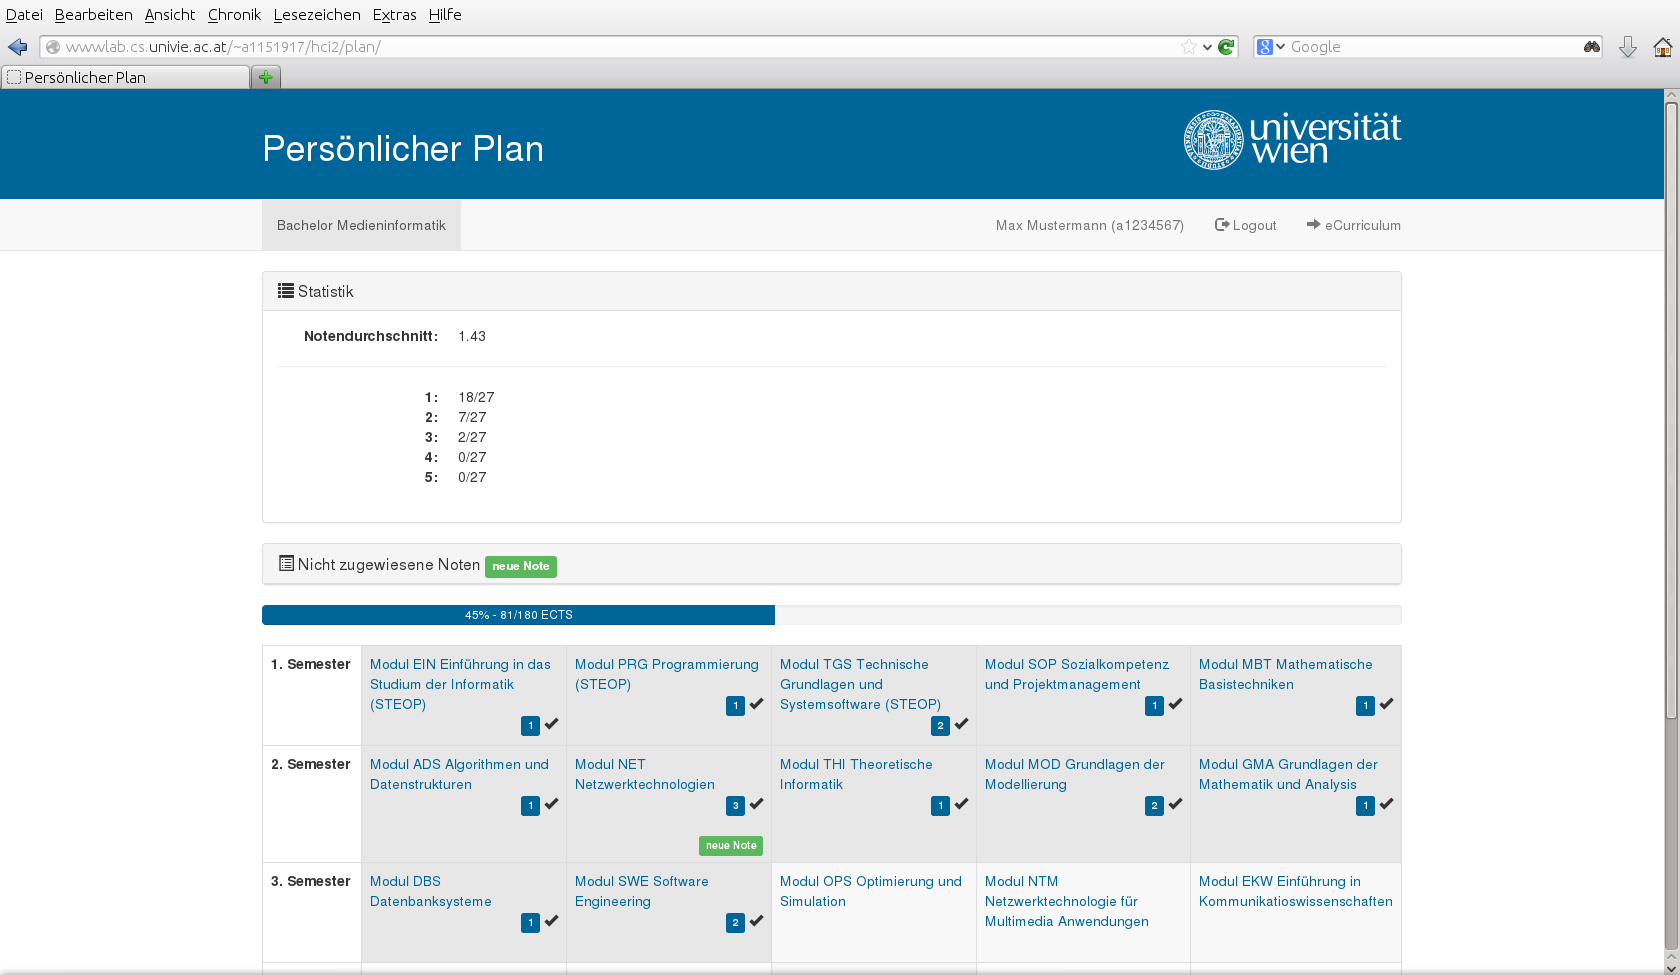
\includegraphics[width=\textwidth]{./verbesserung1.png}}
\medskip

\subsubsection*{Verlinkung zur Anmeldung zur Lehrveranstaltung}

Wenn eine Lehrveranstaltung noch nicht absolviert wurde, wird direkt ins Vorlesungsverzeichnis zum jeweiligen Modul verlinkt.

\noindent\makebox[\textwidth]{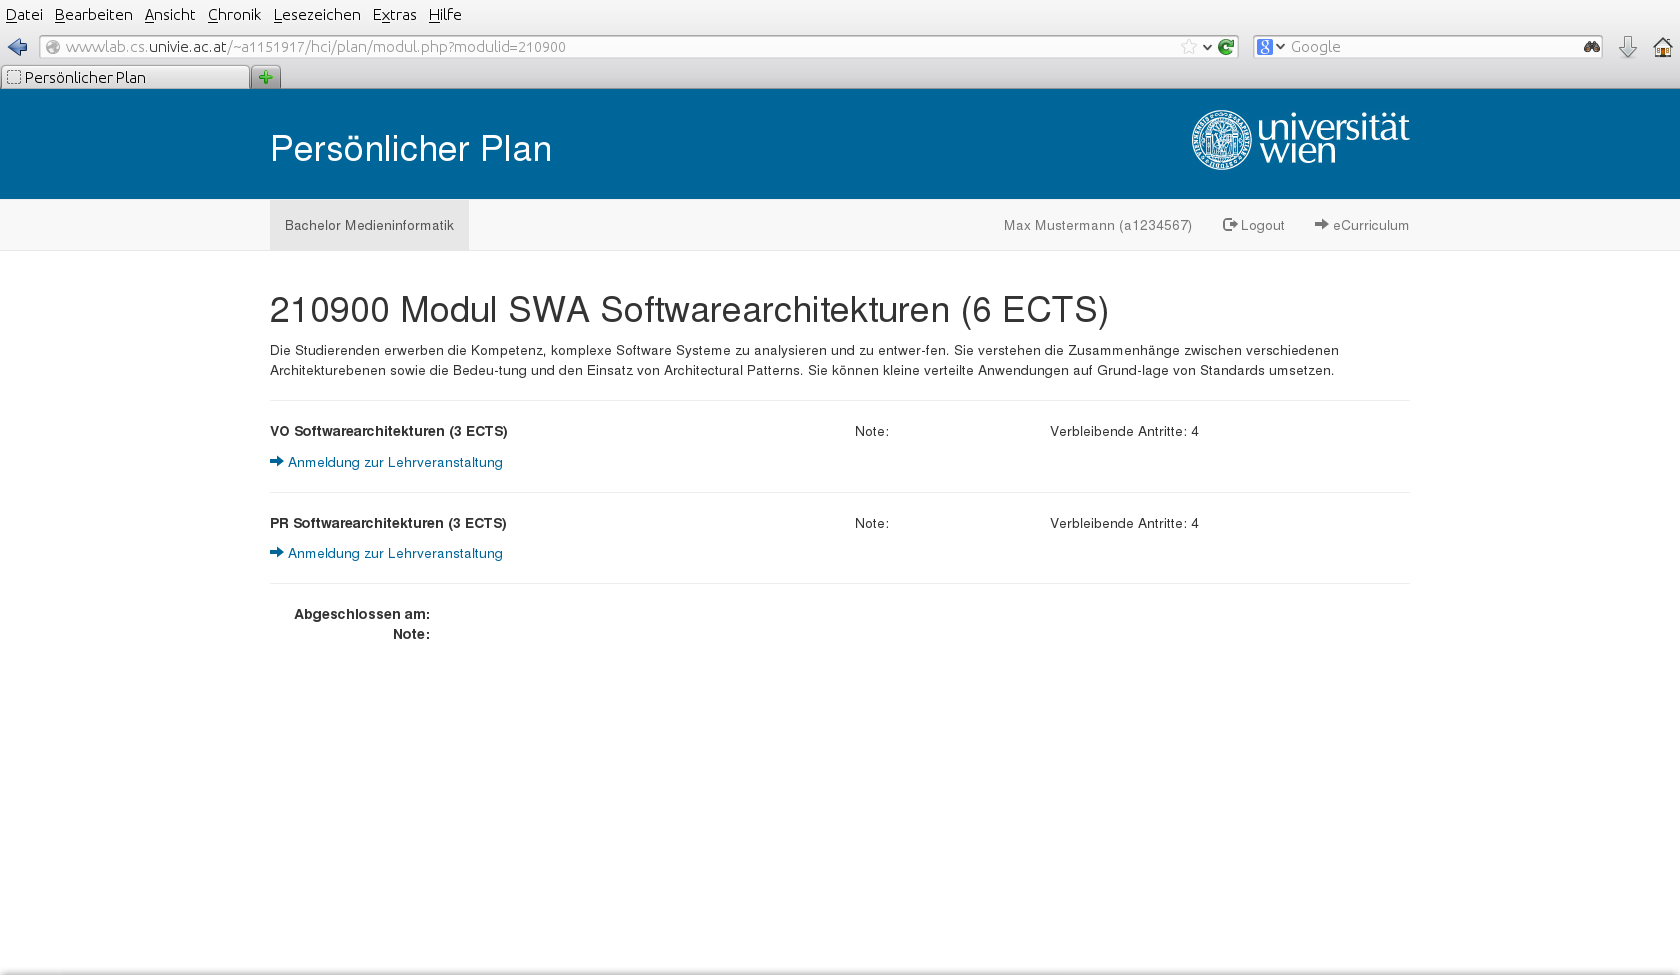
\includegraphics[width=\textwidth]{./verbesserung2.png}}
\medskip

\subsubsection*{Aufklappen aller Module im eCurriculum}




\subsection{Weiterentwicklung nach dem Interview}

\end{document}
